\section{Approach}
	In this section we will present our aproach to tackle the speaker recognition problem.
	There're two steps in a complete speaker recognition system: enrollment and recognition.

\subsection{Erollment}
	\label{sec:approach_enrollment}
	An utterance of a user is collected during enrollment procedure.
	Further processing of the utterance follows following steps:
	\begin{enumerate}
		\item \textbf{VAD} \\
            Signals must be first filtered to rule out the silence part, otherwise the
            training might be seriously biased. Therefore \textbf{Voice Activity Detection} must
            be first performed.
			An observation found is that, the corpus provided is nearly noise-free.
            Therefore we use a simple energy-based approach
			to remove the silence part, by simply remove the frames that the average
            energy is below 0.01 times the average energy of the whole utterance.

            This energy-based method is found to work well on database, but not
            on GUI. We use LTSD(Long-Term Spectral Divergence) \cite{ltsd1} algorithm on GUI, as well as
            noise reduction technique from SOX\cite{sox} to gain better result.

		\item \textbf{MFCC and LPC Features} \\ We extract
          \textbf{Mel-frequency cepstral coefficients} and \textbf{Linear Predictive
			Coding} features using following parameter are found to be
			optimal, according to our experiments in \secref{result}:

			\begin{itemize}
				\item Common parameters:
					\begin{itemize}
						\item Frame size: 32ms
						\item Frame shift: 16ms
						\item Preemphasis coefficient: 0.95
					\end{itemize}
				\item MFCC parameters:
					\begin{itemize}
						\item number of cepstral coefficient: 15
						\item number of filter banks: 55
						\item maximal frequency of the filter bank: 6000
					\end{itemize}
				\item LPC Parameters:
					\begin{itemize}
						\item number of coefficient: 23
					\end{itemize}
			\end{itemize}

			and then concatenate the two feature vectors of the same frame forming
			a larger feature vector of 15 + 23 = 38 dimension.

		\item \textbf{GMM}

			We use \textbf{Gaussian Mixture Model} modeling a speaker. Some improvements made:
			\begin{itemize}
				\item Performance: \\
					We investigate the effect of initialization of GMM during
					training. We implemented GMM with
					K-meansII\cite{bahmani2012scalable}, which is an improved
					version of K-means++\cite{arthur2007k} to initialize the
					mean vector of GMM. Results shows improvements compared
					to GMM provided by \textbf{scikit-learn\cite{scikit-learn}}.
				\item Efficiency:
					\begin{itemize}
						\item We provide a parallel version of GMM, especially
							optimized to train large Universal Background Model(UBM).
						\item We further improve efficiency by utilizing
							SSE instruction in computing exponential function
							using polynomial approximation. This can speed up
							the training procedure by a factor of two.
					\end{itemize}
                \end{itemize}

		\item \textbf{UBM}

			As we are providing continuous speech close-set diarization function in
			GUI, we adopt \textbf{Universal Background Model} as imposter model,
			and use likelihood ratio test to make reject
			decisions.\cite{reynolds2000speaker}

			When using conversation mode in GUI (will be present later),
			GMM model of each user is adapted from a pre-trained UBM
			using method described in \cite{reynolds2000speaker}.

		\item \textbf{CRBM}

          \textbf{Restricted Boltzmann Machine} is generative stochastic
		  two-layer neural network (see \figref{rbm}) that can learn a probability distribution
			over its set of binary inputs\cite{rbm_wiki}.  \textbf{Continuous
			restricted Boltzmann Machine(CRBM)}\cite{chen2003continuous} extends
			its ability to real-valued inputs.  RBM has a ability to, given an
			input(visible layer), reconstruct a visible layer that is similar
			to the input.  \figref{crbm} illustrate original MFCC data and the
			sampled output of reconstructed data from CRBM.

			Previous working using neural network largely focused on speech
			recognition, such as \cite{deep} \cite{mohamed20111deep}, only a
			few (\cite{}) on classification task.

			\begin{figure}[!ht]
				\begin{minipage}{0.48\linewidth}
					\centering
					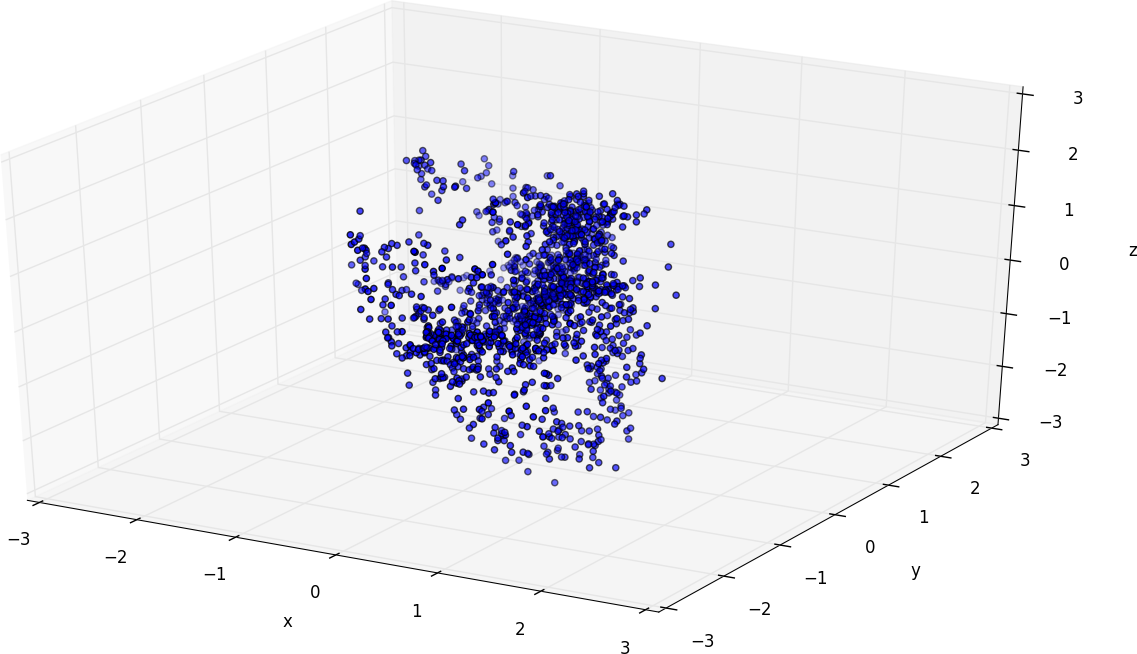
\includegraphics[width=\linewidth]{img/all.trimed.png}
					\caption{The first three dimension of a woman's MFCC feature}
				\end{minipage}
				\hfill
				\begin{minipage}{0.48\linewidth}
					\centering
					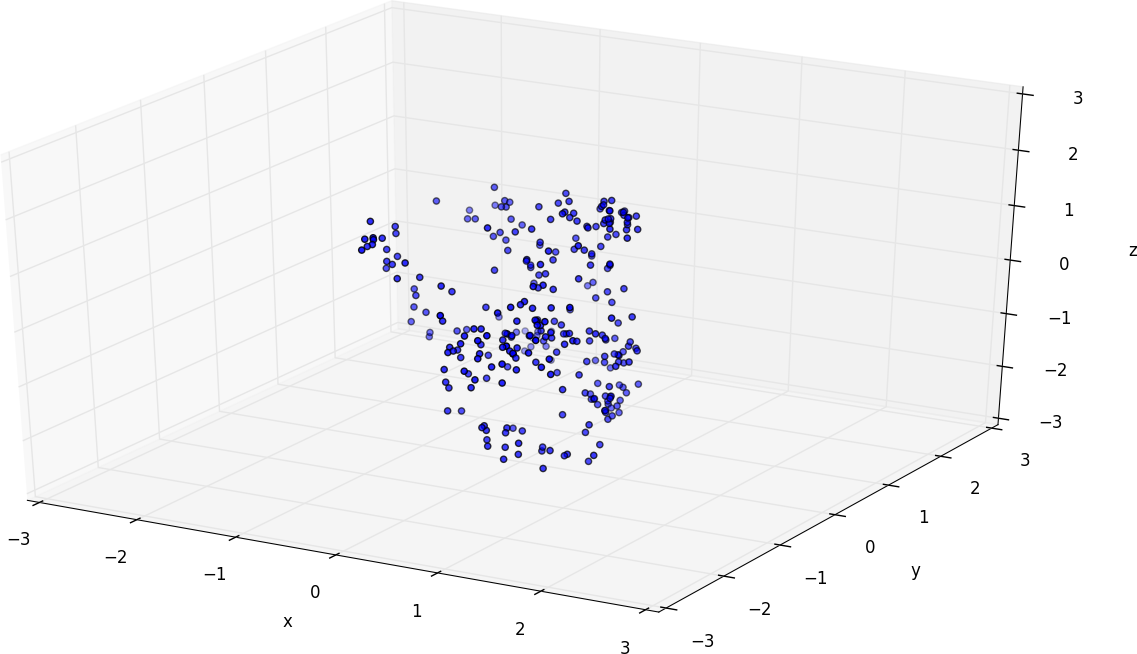
\includegraphics[width=\linewidth]{img/50.trimed.png}
					\caption{The first three dimension of the same woman's MFCC feature
					recontructed by a CRBM with 50-neuron hidden layer. We can
					see that, the density of these two distributions are alike}
				\end{minipage}
                \caption{\label{fig:crbm}}
			\end{figure}

			Here use CRBM as a substitution of GMM, rather than
			an feature extractor. We train a CRBM per speaker,
			and estimate reconstruction error without sampling (which is stable).
			The person corresponds to the lowest reconstruction error CRBM is adopted as
			recognition result.

		\item \textbf{JFA}:

          \textbf{Joint Factor Analysis} \cite{jfa2,jfa-se} was generally considered to perform better than other method
          in the task of Speaker Recognition, by modeling different types of variabilities in the training data, including session variability and
          speaker variability.

          Therefore, we use a simpler algorithm presented in \cite{jfa-study} to train the JFA model.
          However, the result shows that JFA does not seem to outperform GMM.
          We suspected that the training of a JFA model needs more data than
          we provided, since JFA needs data from various source to account for different types of variabilities.
          To get a higher accuracy in JFA, We might need to add extra data for training.
	\end{enumerate}

\subsection{Recognition}
	Recognition procedure follows steps below:
	\begin{enumerate}
		\item Record a short utterance of the speaker (typically less than 5 seconds)

		\item Preprocess the utterance using first two steps described in
			\secref{approach_enrollment}, e.g, VAD, MFCC and LPC feature extraction.

		\item Compute the `score' of each person enrolled, and adopt person
			corresponding the model which gives highest score to be the
			recognition result.

			A typical form of score is log-likelihood (or energy in RBM case).
	\end{enumerate}
